\section{Views}
\label{sec:views}

\subsection{Logic View}
A simple version of the logic view was made because it is hard to foresee all
help classes and states prior to the start of the development process.
\begin{center}
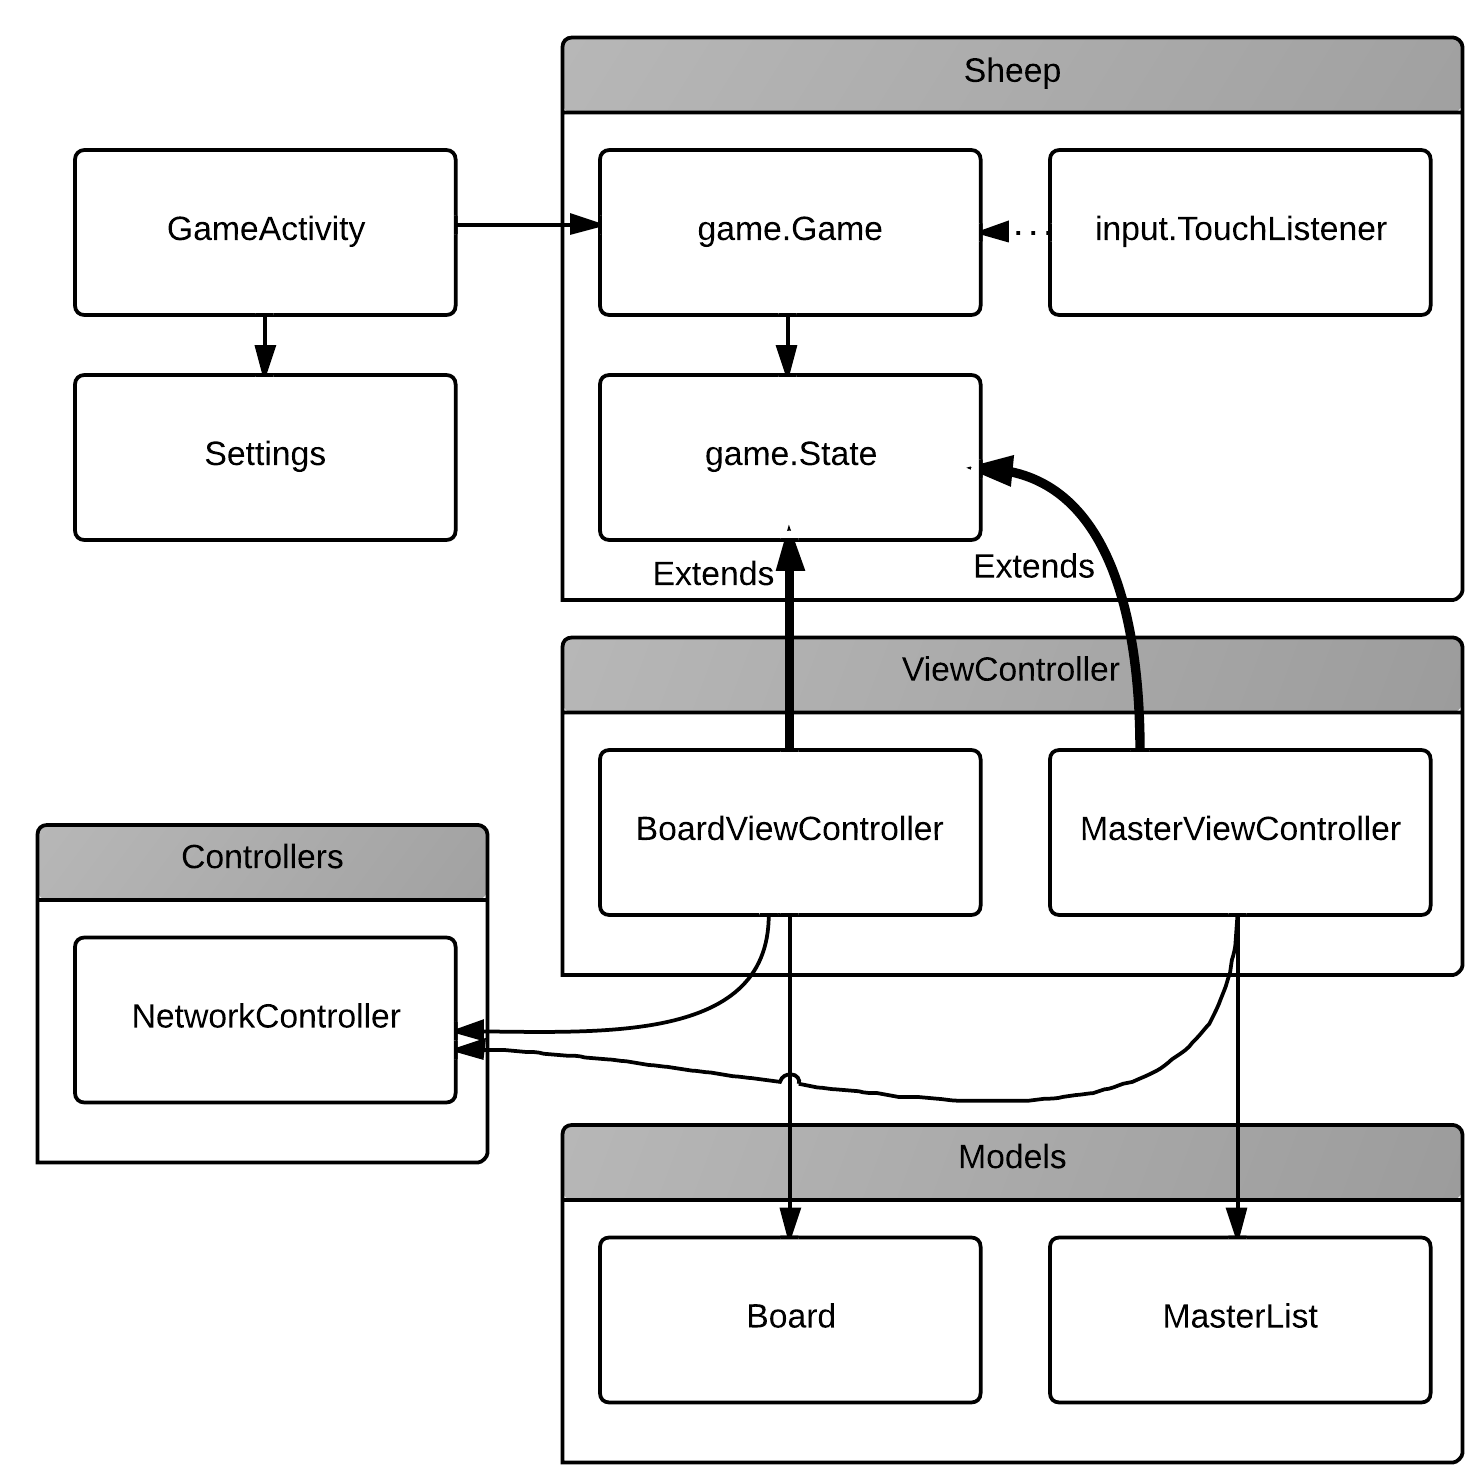
\includegraphics[clip=true, width=0.9 \textwidth]{assets/LogicView.png}
\captionof{figure}{Logic View}
\label{ref:gantt}
\end{center}

\subsection{Development View}
The development view is a hierarchy of layers containing assets such as the
graphics, the game logic (including handling of states and input), the Sheep
framework (which is a typical utility framework) and the Android SDK taking care
of the networking and the base communication with the Android platform.
\begin{center}
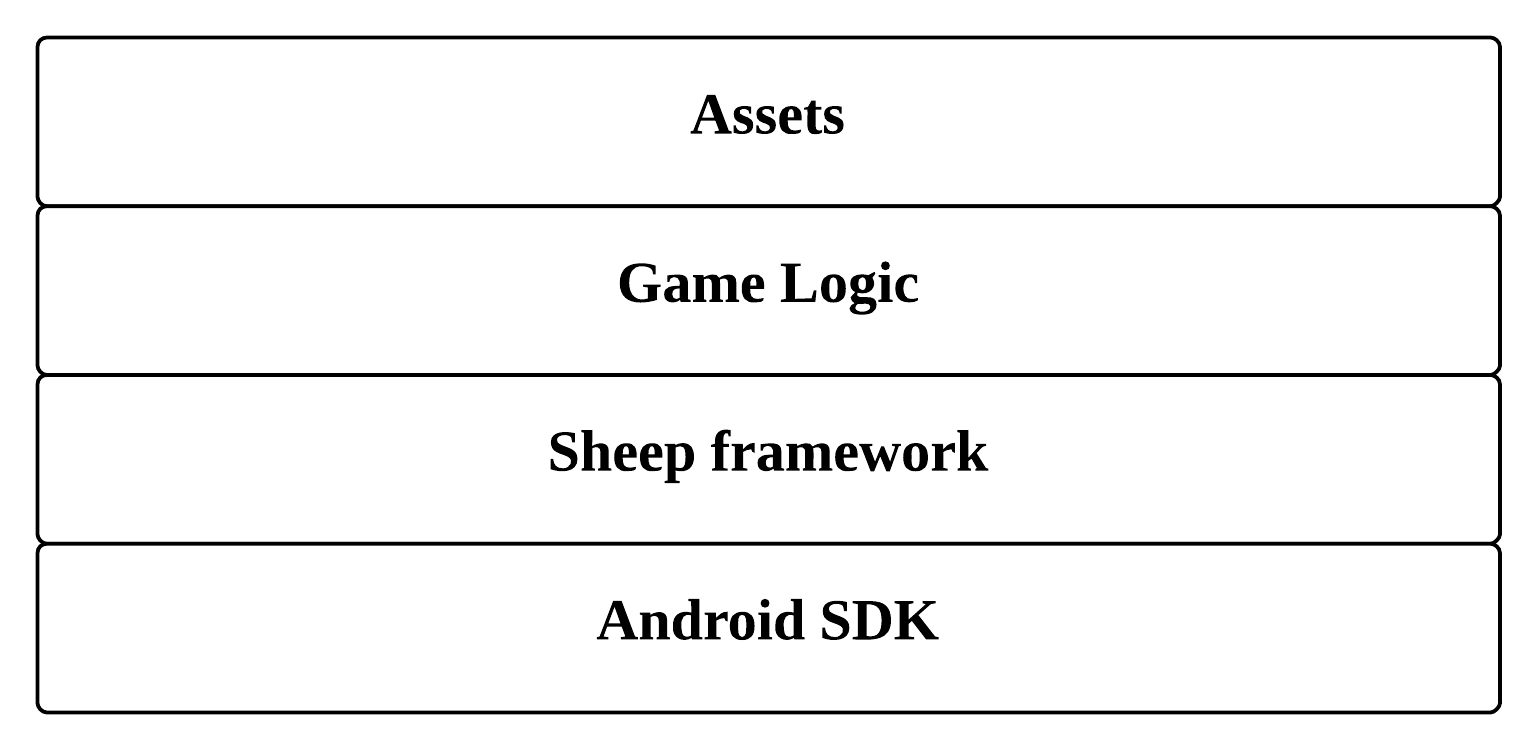
\includegraphics[clip=true, width=0.9 \textwidth]{assets/DevelopmentView.png}
\captionof{figure}{Development View}
\label{ref:gantt}
\end{center}

\subsection{Process View}
The process view shows the process flow in the game, how connections are made
between states and screens.

The menu screen is the entry point of this application where there are options
to navigate to either the authentication or the settings screens. From the
authentication screen the user can log in to, or out of, the admin screen.

The main menu also provides the option to join a new game. If this option is
chosen, the user is transferred to the game screen, which has listeners for
notification states. The game ended screen returns to the main menu.
\begin{center}
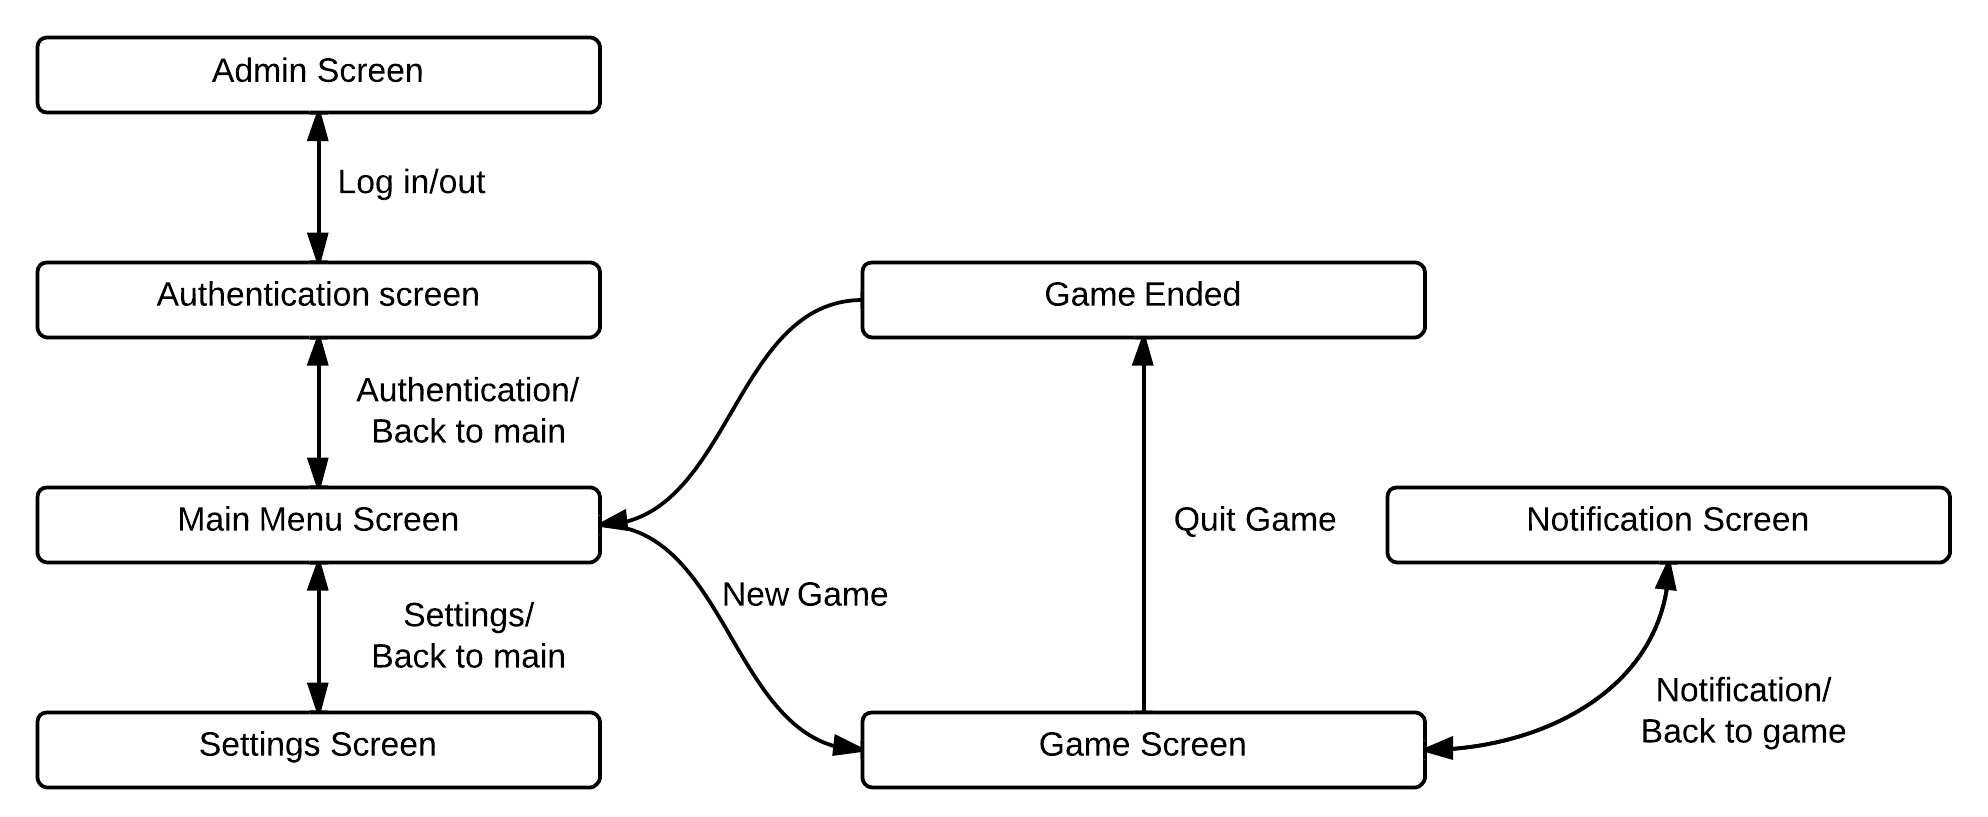
\includegraphics[clip=true, width=0.9 \textwidth]{assets/ProcessView.png}
\captionof{figure}{Process View}
\label{ref:gantt}
\end{center}

\subsection{Physical View}
\begin{center}
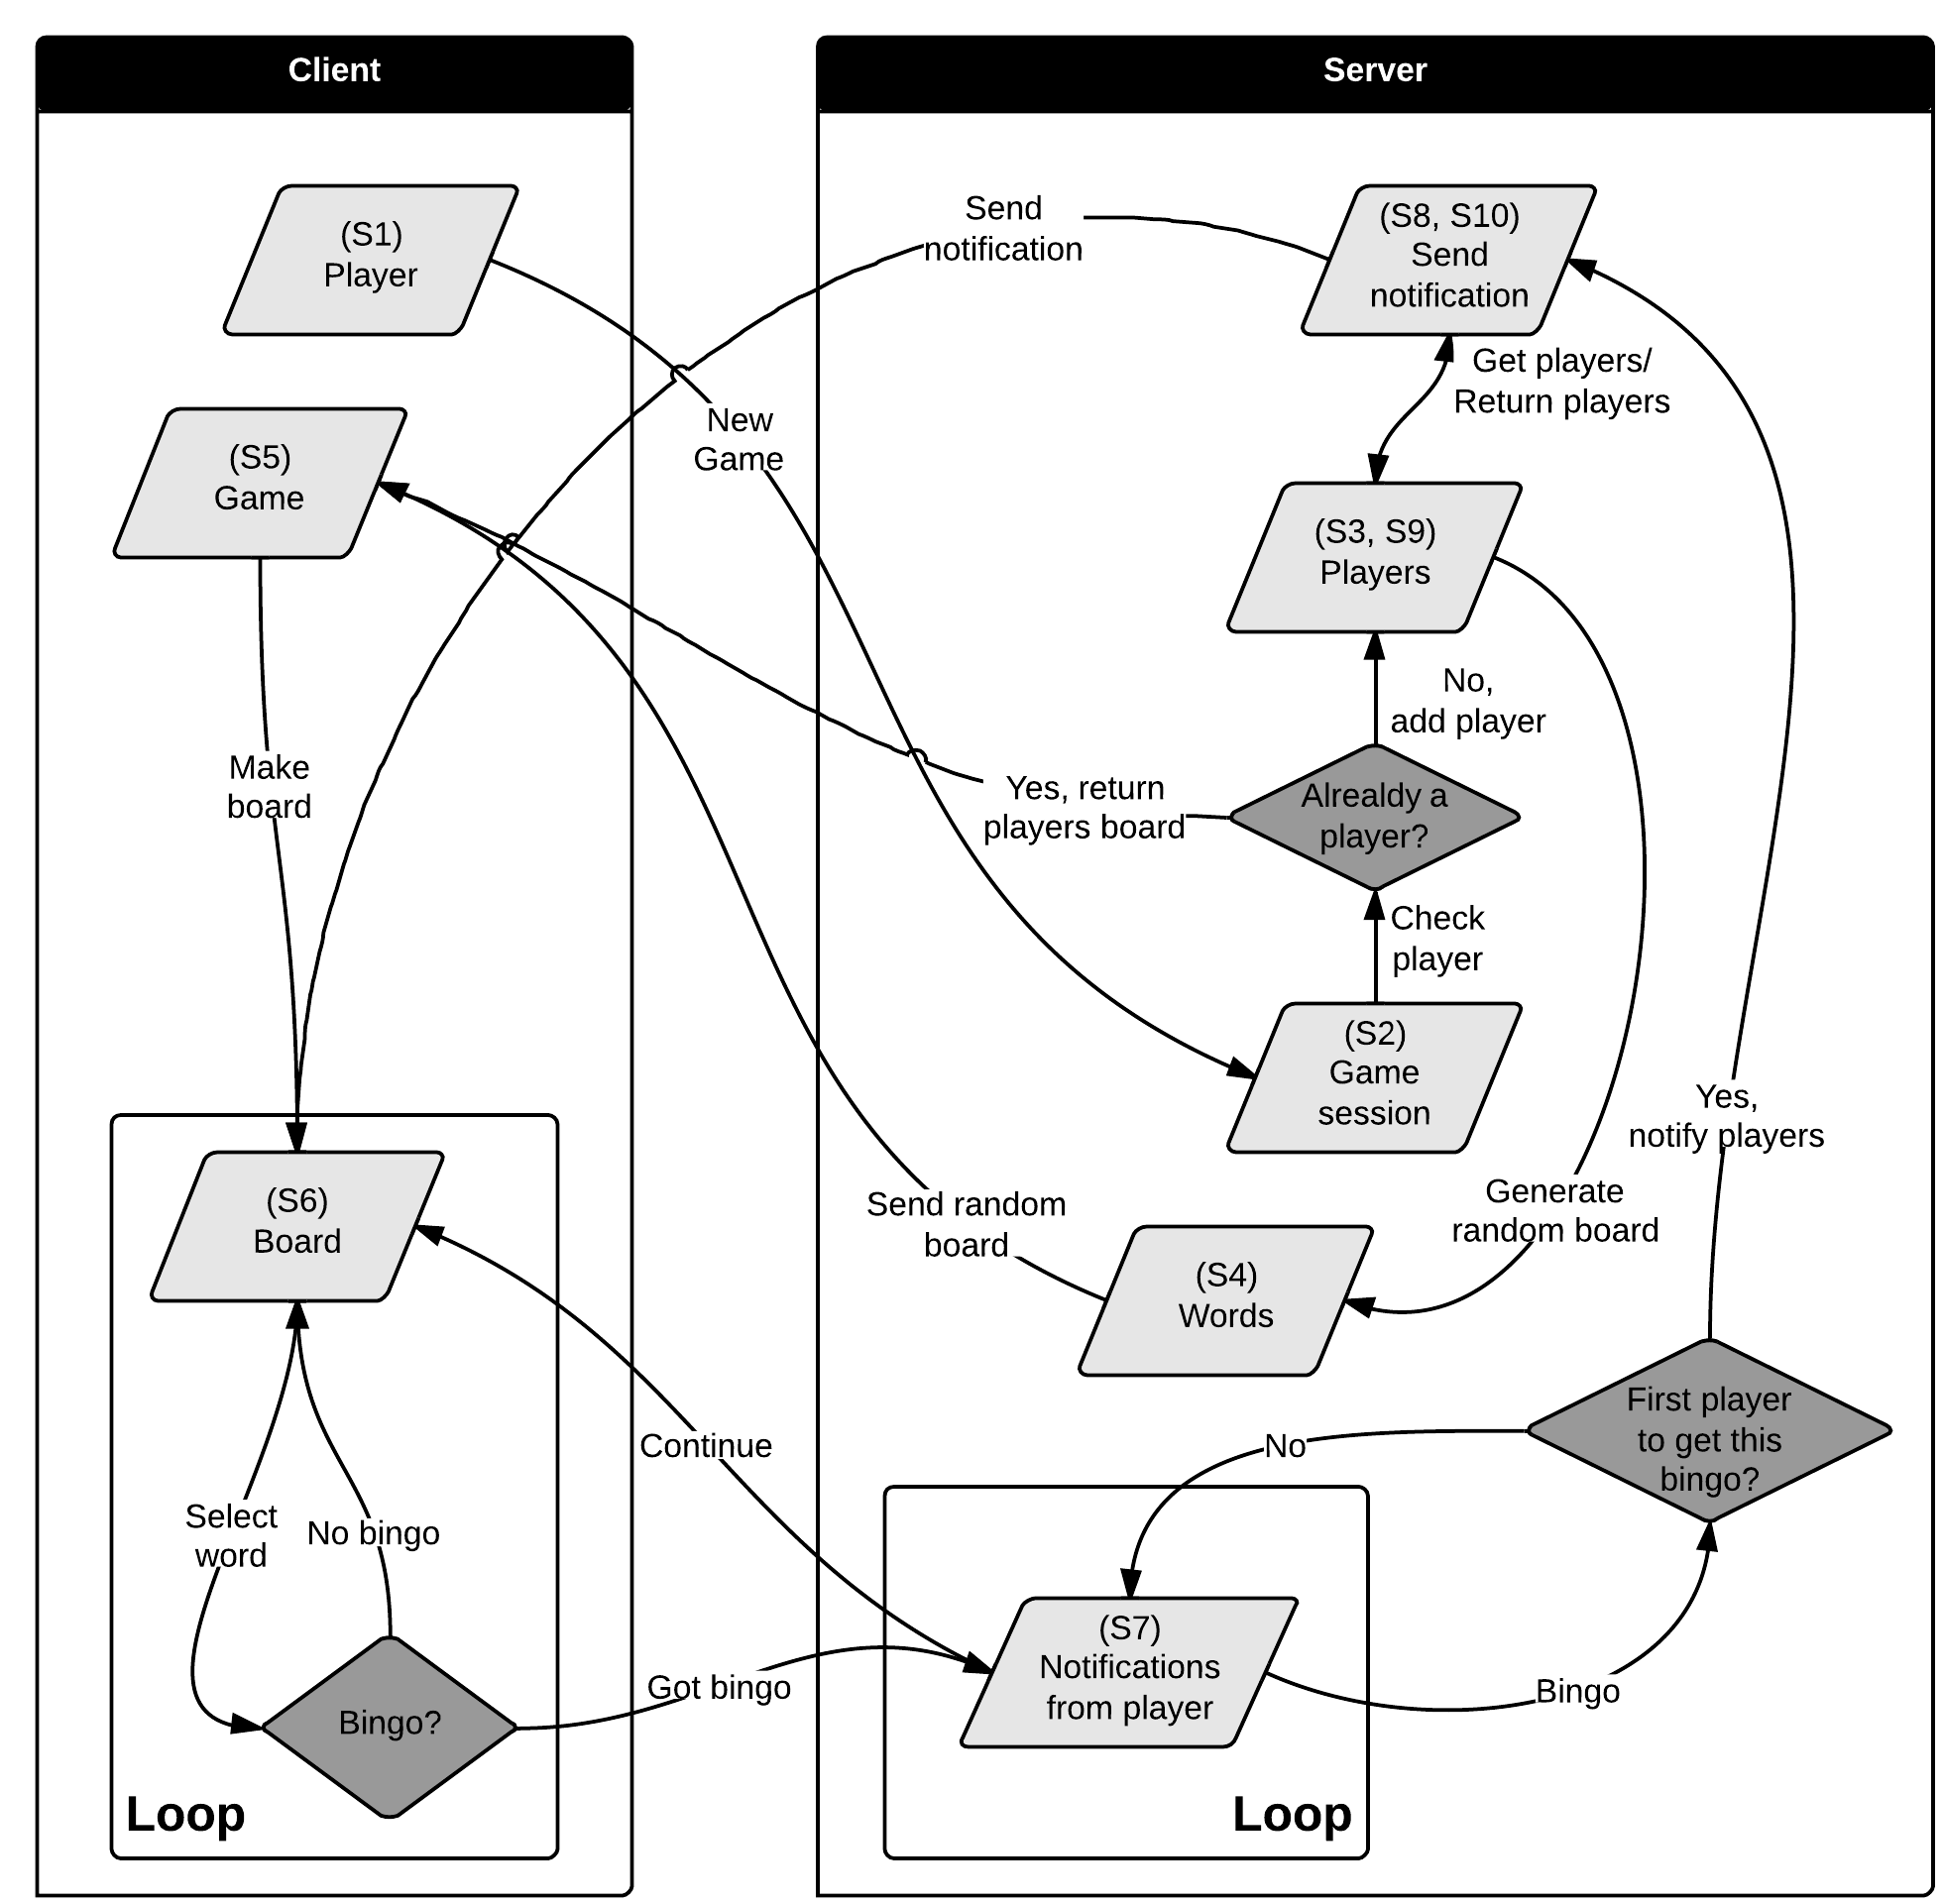
\includegraphics[scale=0.5]{PhysicalViewFinal}
\captionof{figure}{Physical view for Bedpres Bingo}
\end{center}

The system in parted into two subsystems which communicate. The client is the Android application and the server is our server instance which may run on any PC with python. 

The different states and how they relate are shown in the diagram. 
When a player starts, they initiate a new game(S1). This will make a call to the server(S2), which checks if the player already has a game. If no, the player is added and is added to the list of active players(S3). If yes, the player recieves their old game board(S5). 

When the server adds the player in (S3), a random game board is generated(S4) and the board is sent to the player(S5).
From the words recieved, a board is made on the Android application (S6). In (S6) the player is in a loop when selecting words. If the word selected results in a bingo, a notification is sent to the server(S7). In (S7) a check is done to check if the player is the first one to get a bingo. If the player is the first one to achieve a bingo a notification is sent to the other players(S10).

\subsection{Consistency among views} 
\label{sec:consistencyamongviews}
%TODO: Update when finished

Apart from the develompent view not showing specifically what goes under client
or server, the views are consistent. In the development view the server is
under the Game Logic, and networking is under the SDK\@.

Apart from this, the other views and relations are consistent.
